\chapter{This Land Is My Land}

These companion notes follow Michael Sandel's fourth lecture in the \textit{Justice} course, as curated in the LazyLearn track by LazyingArt LLC. The lecture begins by making Locke look like a natural ally of libertarianism and then steadily complicates that first impression. We move from natural rights to the state of nature, from the state of nature to private property, and from private property to consent, only to end with a more difficult question: if consent matters so much, what work does it actually do once natural rights and majority rule are both in place?

\section{Locke as the Apparent Libertarian Ally}

Sandel opens by giving Locke his strongest possible libertarian appearance. Locke affirms fundamental individual rights so important that no government may override them, not even a representative or democratically elected one. And the set of rights at issue is not narrow. It includes life, liberty, and property.

It is useful to summarize the opening claim schematically:
\begin{align}
R_{\mathrm{nat}} &= \{\text{life},\ \text{liberty},\ \text{property}\},\\
\text{property is a natural right} &\Longrightarrow \text{property is pre-political in principle.}
\end{align}

This is the first major frame of the lecture. Property is not introduced as a legal artifact created by legislatures. It is introduced as something that attaches to persons as human beings, even before law and government arrive on the scene. That immediately forces the next question. If rights are natural in this sense, what would the world look like before institutions exist to define and enforce them? Locke's answer is the state of nature.

\section{State of Nature: Liberty, Not License}

The state of nature is not for Locke a piece of anthropology and not yet a doctrine of chaos. It is a conceptual device for asking what rights mean before government. Sandel emphasizes two features at once: people are free and equal in the state of nature, and yet that freedom is not unlimited.

The lecture's first sharp distinction can be written as
\begin{equation}
\text{State of Nature}=\text{Liberty}\neq \text{License}.
\end{equation}

The first half of the formula matters because Locke denies natural hierarchy. No one is born to rule and no one is born to serve. The second half matters just as much, because freedom here does not mean a permission to do whatever we want. Even before there is positive law, there is still a law of nature.

\subsection{Question \& Answer}

\paragraph{Question.} If we are free and equal in the state of nature, why are we not free to do whatever we want?

\paragraph{Answer.} Because the state of nature contains a moral constraint internal to it. Freedom means the absence of natural political superiors, not the absence of all norm. Sandel compresses Locke's point into a pair of prohibitions: we may not give up our own natural rights, and we may not violate those of another. Schematically,
\begin{equation}
\neg \text{alienate one's own natural rights},
\qquad
\neg \text{violate another's natural rights}.
\end{equation}

That is why the lecture can say both that we are free and that we are not free to kill, enslave, or subject either ourselves or others to arbitrary absolute power. The state of nature is already morally structured.

\section{Unalienable Rights and Their Two Foundations}

Once the distinction between liberty and license is in place, Sandel asks the next necessary question: where does the constraint come from? He gives Locke's two answers in sequence.

The first answer is theological. Human beings are the workmanship of God, and therefore God's claim on us precedes our discretionary power over ourselves. As a schematic shorthand,
\begin{equation}
\text{God's prior property right in us} > \text{our discretionary power over ourselves}.
\end{equation}

This first answer explains why we are not fully at liberty to dispose even of our own lives and liberties. But Sandel does not stop there. He immediately asks what Locke can say to those who do not begin from theology, and that brings in the second answer: reason.

Here the lecture moves from divine workmanship to rational reflection:
\begin{align}
\text{Reason} &= \text{Law of Nature},\\
\forall x\neq y,\quad x &\text{ ought not harm } y \text{ in life, health, liberty, or possessions.}
\end{align}

This is the point at which Sandel introduces the paradox of unalienable rights. In one familiar sense, a non-transferable right is less fully mine: I cannot sell it, trade it, or dispose of it at will. The airline-ticket analogy makes that clear. But in the more morally weighty sense that Locke and Jefferson care about, an unalienable right is more deeply mine. It is so essentially bound up with my standing as a person that even I cannot give it away.

This is why unalienability distances Locke from a crude doctrine of absolute self-ownership. If our rights are truly natural, then taking them seriously does not yield the conclusion that we may do anything we please with ourselves. It yields the opposite conclusion: that some of our most fundamental rights are precisely not at our disposal.

\section{Property Before Government: From Person to Labor to Land}

Sandel now turns from rights in general to the lecture's central constructive argument. The difficult question is not whether life and liberty can be natural rights; it is whether private property can arise even before government exists to define and enforce ownership.

Locke's answer in Section 27 begins with the person:
\begin{equation}
\text{property in person}\to \text{property in labor}\to \text{mix labor with the unowned}\to \text{private property}.
\end{equation}

This is the labor theory of appropriation in its cleanest form. The argument proceeds step by step, and Sandel is careful not to skip any of them.

\paragraph{Worked derivation.}
\begin{enumerate}
\item Each person has a property in his own person.
\item The labor of his body and the work of his hands are therefore properly his.
\item Let \(o\) be something unowned and left in common.
\item If a person's labor is mixed with \(o\), then \(o\) is no longer merely common in the same way it was before.
\item Since the labor is already the laborer's own, the resulting claim can become a private one.
\end{enumerate}

We can write the same movement in compact form:
\begin{equation}
o\in U,\qquad \text{mix }L_x\text{ with }o \Longrightarrow o\in P_x,
\end{equation}
where \(U\) names what nature has left in common, \(L_x\) the labor of person \(x\), and \(P_x\) what belongs to \(x\). This is only a schematic reconstruction, but it captures the logic Sandel attributes to Locke.

\paragraph{A worked example.}
Suppose an apple lies in the common stock \(U\). If person \(x\) picks it, then the apple is no longer merely where nature left it. It has been joined to labor that is already \(x\)'s. In that case the apple may become \(x\)'s property.

Locke then presses the stronger claim. If the object is not just an apple but a parcel of land, and if that land is tilled, planted, improved, cultivated, and enclosed, the claim extends beyond the crop to the land itself:
\begin{equation}
\text{till}+\text{plant}+\text{improve}+\text{cultivate}
\Longrightarrow
\text{property not only in crop but in land.}
\end{equation}

This is a much stronger move than the simple acorn or apple case. It turns labor not merely into a title over what one gathers, but into a title over the earth one has worked.

Yet Locke's argument is not unrestricted. It is governed by the famous proviso:
\begin{equation}
\text{valid appropriation}\Longrightarrow \text{``enough and as good'' left for others.}
\end{equation}

So the lecture's constructive chain has two parts. First, labor can generate private claims. Second, those claims are valid only under a condition that preserves room for others.

\subsection{Question \& Answer}

\paragraph{Question.} How can private property arise before government or consent?

\paragraph{Answer.} Locke's answer is that consent is not needed for the original act of appropriation. The crucial moral bridge is labor. We begin from property in the person, pass to property in labor, and then treat labor mixed with the unowned as sufficient to generate ownership. Government arrives later, not to create the very possibility of property, but to stabilize and define it in a civil setting.

\section{Testing Locke's Property Argument: Patents, Colonization, and Common Use}

Sandel does not leave the labor theory at the level of tidy formula. He tests it with examples. The first is contemporary: the dispute over drug patents during the AIDS crisis in South Africa. The moral intuition behind the patent claim is recognizably Lockean. A pharmaceutical company invests labor, research, and ingenuity into developing a drug; why should that product not be theirs?

At the same time, the case already exposes a difficulty. The South African government seeks cheap generic drugs in order to save lives. So labor, need, and public good all collide. Sandel uses the case not as a direct application of Locke's theory to intellectual property, but as an intuition pump. It keeps alive the thought that creation can matter morally for ownership, while also showing that questions of property quickly become questions about rules, institutions, and human consequences.

He then sharpens the challenge historically. The classroom exchange about Native Americans and European settlement asks whether Locke's theory is a justification or a rationalization. Rochelle's worry is direct: if the labor theory validates enclosure, then it may have served to legitimate colonial appropriation. Sandel frames the issue starkly. If the argument is sound, it would justify that appropriation; if it is unsound, it is mere rationalization.

The replies matter. Dan points out that use itself may count as labor. If hunting, gathering, or sustained use already involve labor, then the Native Americans may have had claims within Locke's own framework. Fang adds a second point: if land is used in common, and if the proviso requires enough and as good to remain, then easy colonial enclosure becomes even harder to justify. Sandel does not resolve the issue neatly. He uses the exchange to show that the theory of appropriation is morally unstable precisely where history makes it most consequential.

\section{Consent as the Second Big Idea}

After the lecture's recap-style reset, Sandel names consent as Locke's second big idea. Property is one large theme; consent is the other. To understand what consent does, we must return to the state of nature and ask why anyone would ever leave it.

Locke's answer is not that the state of nature lacks rights. It is that the enjoyment of those rights is insecure because everyone may enforce the law of nature for himself or herself. Everyone is, as Locke says, an executor of the state of nature. Since each person becomes judge in his or her own case, punishment overshoots and insecurity spreads.

The lecture's transition can be summarized as
\begin{equation}
\text{everyone enforces law of nature}
\to
\text{punishment overshoots}
\to
\text{insecurity}
\to
\text{consent to civil society}.
\end{equation}

And the crucial point is that what is surrendered is not the rights themselves but the private power of enforcement:
\begin{equation}
\text{consent}\Longrightarrow \text{surrender private enforcement power},
\qquad
\text{not}\Longrightarrow \text{surrender natural rights}.
\end{equation}

\begin{figure}[h]
\centering
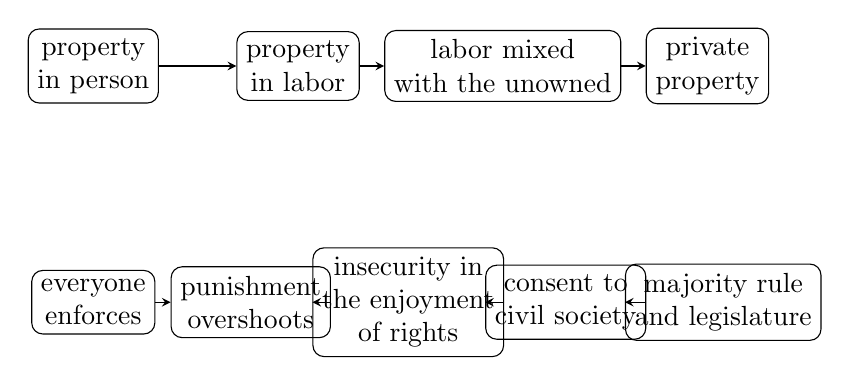
\begin{tikzpicture}[>=stealth]
\node[draw, rounded corners, align=center] (p1) at (0,1.6) {property\\in person};
\node[draw, rounded corners, align=center] (p2) at (2.6,1.6) {property\\in labor};
\node[draw, rounded corners, align=center] (p3) at (5.2,1.6) {labor mixed\\with the unowned};
\node[draw, rounded corners, align=center] (p4) at (7.8,1.6) {private\\property};

\draw[->] (p1)--(p2);
\draw[->] (p2)--(p3);
\draw[->] (p3)--(p4);

\node[draw, rounded corners, align=center] (c1) at (0,-1.4) {everyone\\enforces};
\node[draw, rounded corners, align=center] (c2) at (2.0,-1.4) {punishment\\overshoots};
\node[draw, rounded corners, align=center] (c3) at (4.0,-1.4) {insecurity in\\the enjoyment\\of rights};
\node[draw, rounded corners, align=center] (c4) at (6.0,-1.4) {consent to\\civil society};
\node[draw, rounded corners, align=center] (c5) at (8.0,-1.4) {majority rule\\and legislature};

\draw[->] (c1)--(c2);
\draw[->] (c2)--(c3);
\draw[->] (c3)--(c4);
\draw[->] (c4)--(c5);
\end{tikzpicture}
\caption{Two schematic chains that organize the lecture: the labor theory of appropriation and the transition from private enforcement to civil society.}
\end{figure}

\subsection{Question \& Answer}

\paragraph{Question.} If natural rights remain in force, what exactly does consent authorize the majority to do?

\paragraph{Answer.} Consent authorizes the creation of a political community with standing law, a legislature, and a rule of majority decision. What it does not obviously authorize is the violation of the very rights that supposedly survive entry into society. This is why the lecture's second half becomes a puzzle rather than a simple endorsement of majority rule. Consent explains why we leave the state of nature; it does not by itself settle the limits of the powers we create.

\section{Taxation, Implied Consent, Conscription, and Locke's Limits}

The lecture's hardest tension appears when Sandel turns to Locke's own text on taxation. On the one hand, Locke says that the legislature cannot take any part of a man's property without his own consent. On the other hand, when he explains taxation, he identifies that consent with the consent of the majority.

The tension can be written succinctly as
\begin{equation}
\text{no taking of property without consent}
\qquad\text{vs.}\qquad
\text{taxation by consent of the majority}.
\end{equation}

Sandel's reconstruction of the problem is subtle. Locke now seems to say two things at once. Property is natural, because government exists in order to preserve it. But what counts as \emph{mine} within society is also defined by the law of the community. Hence the lecture's synthesis:
\begin{equation}
\text{property as an institution is natural},
\qquad
\text{what counts as mine is conventionally defined}.
\end{equation}

This distinction is the pivot of the second half. The natural right is not to each concrete holding exactly as it stands independent of law; rather, it is to there being an institution of property, and to that institution not being overridden arbitrarily. Once we see that, majority consent begins to do more work than the libertarian had hoped.

The discussion of implied consent then exposes another weakness. Nicola asks what becomes of those born into an existing society. They never literally signed a social contract. The provisional Lockean reply is tacit or implied consent: by using roads, protection, and public institutions, one accepts the political order. Sandel does not treat this as a final victory. He uses the exchange to show how fragile the consent argument becomes when explicit agreement disappears and only inherited membership remains.

\subsection{Question \& Answer}

\paragraph{Question.} Can those who never explicitly consented still be bound by government, taxation, or even conscription?

\paragraph{Answer.} Locke seems to rely on a combination of collective consent and tacit consent. Collective consent enters when the original act of association binds the society to majority rule. Tacit consent enters when those born into society accept its protections and continue to live under its institutions. But Sandel does not present this as a knockdown solution. The very need to appeal to implied consent shows how far Locke is from the simple picture in which each citizen has individually authorized every law that binds him.

The pressure intensifies when the lecture moves from property to life. Military conscription seems harder to justify than taxation, because unalienable rights are supposed to be beyond our power to give away. If I cannot consent to my own enslavement or suicide, how can I be said to have consented to a law that may compel me to fight?

Sandel's likely Lockean answer turns on a final distinction:
\begin{equation}
\text{arbitrary taking}=\text{illegitimate},
\qquad
\text{general non-arbitrary law}\neq \text{arbitrary taking}.
\end{equation}

On this reading, Locke is not saying that government may never burden life, liberty, or property. He is saying that government may not seize them arbitrarily, at pleasure, by singling out this person or that one. A general law, enacted through standing procedures and applied non-arbitrarily, is not the same thing as a king or parliament choosing Bill Gates to finance a war, or choosing one citizen at whim to surrender his life.

This answer is intelligible, but it is not especially comforting to libertarianism. It means that unalienability does not yield absolute self-ownership, and it means that consent, once joined to general law, can authorize a great deal:
\begin{align}
\text{unalienable rights} &\Longrightarrow \text{self-ownership is not absolute},\\
\text{consent}+\text{general law} &\Longrightarrow \text{government may be less limited than libertarians hope}.
\end{align}

Sandel's final diagnosis is therefore double. Locke disappoints the libertarian first because our rights are not fully at our disposal, and second because a legitimate government acting through non-arbitrary law may still tax, regulate, and even conscript. And then the lecture darkens further. The great theorist of consent also produced a theory of private property that did not require consent at all. When Locke says that ``all the world was America,'' the political and colonial background of the theory comes sharply into view.

\section{Summary}

The lecture begins by making Locke look like a firm defender of pre-political rights and ends by showing how unstable that alliance is. The state of nature is a state of liberty but not license. Unalienable rights are constrained first by God's prior claim and then by reason as the law of nature. Private property arises, on Locke's view, through labor mixed with what nature has left in common, though always under the proviso that enough and as good remain for others. Consent then appears as the device by which we escape the violence of private enforcement and create civil society.

But the deeper result is not a simple vindication of libertarianism. Once majority rule, taxation, implied consent, and conscription enter the picture, Locke's limited government looks less limited than it first seemed. The lecture therefore closes, quite deliberately, on an open problem: if consent is neither everything nor nothing, what is its moral force, and where are its limits? That question now passes from government to markets, which is where the course turns next.